\documentclass[addpoints,spanish, 12pt,a4paper]{exam}
%\documentclass[answers, spanish, 12pt,a4paper]{exam}
\printanswers
\pointpoints{punto}{puntos}
\hpword{Puntos:}
\vpword{Puntos:}
\htword{Total}
\vtword{Total}
\hsword{Resultado:}
\hqword{Ejercicio:}
\vqword{Ejercicio:}

\usepackage[utf8]{inputenc}
\usepackage[spanish]{babel}
\usepackage{eurosym}
%\usepackage[spanish,es-lcroman, es-tabla, es-noshorthands]{babel}


\usepackage[margin=1in]{geometry}
\usepackage{amsmath,amssymb}
\usepackage{multicol}
\usepackage{yhmath}

\pointsinrightmargin % Para poner las puntuaciones a la derecha. Se puede cambiar. Si se comenta, sale a la izquierda.
\extrawidth{-2.4cm} %Un poquito más de margen por si ponemos textos largos.
\marginpointname{ \emph{\points}}

\usepackage{graphicx}

\graphicspath{{../../img/}} 

\newcommand{\class}{2º Bachillerato CIT}
\newcommand{\examdate}{\today}
\newcommand{\examnum}{Global}
\newcommand{\tipo}{A}


\newcommand{\timelimit}{90 minutos}

\renewcommand{\solutiontitle}{\noindent\textbf{Solución:}\enspace}


\pagestyle{head}
\firstpageheader{
\includegraphics[width=0.2\columnwidth]{header_left}}{\textbf{Departamento de Matemáticas\linebreak \class}\linebreak \examnum}{
\includegraphics[width=0.1\columnwidth]{header_right}}
\runningheader{\class}{\examnum}{Página \thepage\ of \numpages}
\runningheadrule


\usepackage{pgf,tikz,pgfplots}
\pgfplotsset{compat=1.15}
\usepackage{mathrsfs}
\usetikzlibrary{arrows}


\begin{document}

\noindent
\begin{tabular*}{\textwidth}{l @{\extracolsep{\fill}} r @{\extracolsep{6pt}} }
\textbf{Nombre:} \makebox[3.5in]{\hrulefill} & \textbf{Fecha:}\makebox[1in]{\hrulefill} \\
 & \\
\textbf{Tiempo: \timelimit} & Tipo: \tipo 
\end{tabular*}
\rule[2ex]{\textwidth}{2pt}
Esta prueba tiene \numquestions\ ejercicios. La puntuación máxima es de \numpoints. 
La nota final de la prueba será la parte proporcional de la puntuación obtenida sobre la puntuación máxima. 

\begin{center}


\addpoints
 %\gradetable[h][questions]
	\pointtable[h][questions]
\end{center}

\noindent
\rule[2ex]{\textwidth}{2pt}

\begin{questions}

%\question 
%
%\begin{parts}
%\part[2] 
%\begin{solution}
%\end{solution}
%


% junio 19





\question[4] Considere la función: $f(x)=\dfrac{x-1}{(x+1)^2}$
\begin{parts}
    \part Determine las asíntotas de la función, si existen
    \part Determine los intervalos de crecimiento y decrecimiento de esa función, si existen
    \part Determinte la integral $\int_{1}^{3} f(x)\ dx$
\end{parts}

\begin{solution}
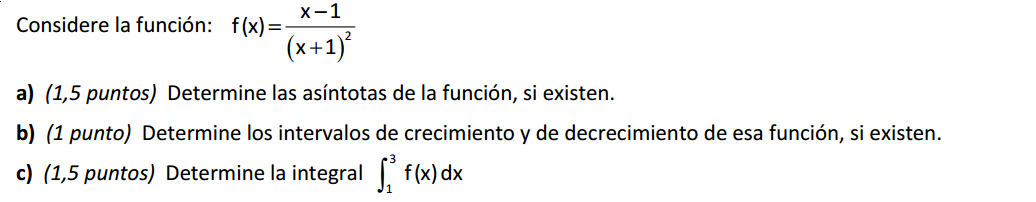
\includegraphics[width=1\textwidth]{2bac/2bac_cie/img/cieju19.png}
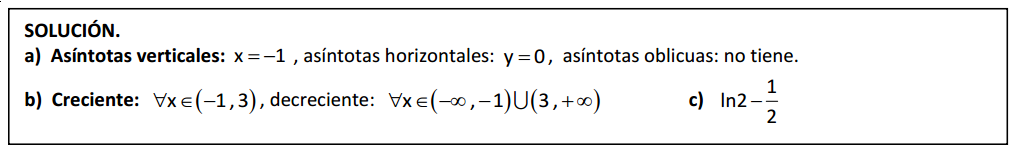
\includegraphics[width=1\textwidth]{2bac/2bac_cie/img/ciejun19sol.png}
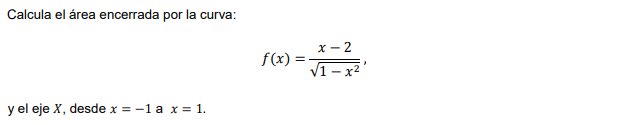
\includegraphics[width=1\textwidth]{2bac/2bac_cie/img/cieres22.png}
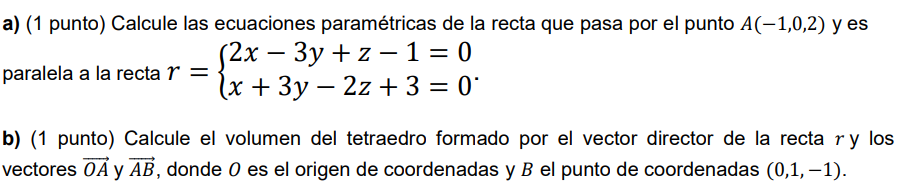
\includegraphics[width=1\textwidth]{2bac/2bac_cie/img/cieresgeo.png}
\end{solution}


\question[4] Calcula el área encerrada por la curva: $$f(x)=\dfrac{x-2}{\sqrt{1-x^2}}$$ y el eje $X$, desde $x=-1$ a $x=1$
\begin{solution}
    $- \sqrt{1 - x^{2}} - 2 \operatorname{asin}{\left(x \right)} \to 2\pi$    
\end{solution}


% \question[4] Determina $b$ sabiendo que $b>0$                                                            y que el área de la región limitada por la curva $y={{x}^{2}}$ y la recta $y=bx$ es igual a $\frac{9}{2}$
% \begin{solution}
%     $\dfrac{b^3}{6}=\dfrac{9}{2} \to b=3$
% \end{solution}

% \question[3] Tres laboratorios producen el 35\% (laboratorio A), 25\% (laboratorio B) y 40\% (laboratorio C) del total
% de los medicamentos que se reciben en la farmacia de un hospital de nuestra comunidad autónoma.
% Además, entre esos medicamentos están las vacunas para la gripe común: el 3\% de los
% medicamentos del laboratorio A son vacunas para la gripe común, el 2\% de los medicamentos del
% laboratorio B son vacunas para la gripe común y el 2\% de los medicamentos del laboratorio C son
% vacunas para la gripe común.
% \begin{parts}
%     \part Si se selecciona un medicamento al azar, calcule la probabilidad de que sea una
% vacuna para la gripe común.
%     \part Si se selecciona una vacuna para la gripe común, calcule la probabilidad de que
% pertenezca al laboratorio C
% \end{parts}

\question[3] Disponemos de los siguientes datos sobre el uso de nuevas tecnologías por parte de los estudiantes de una universidad: un 70\% de los estudiantes de esa universidad tiene teléfono inteligente, un 50\% de los estudiantes de esa universidad tiene ordenador portátil y un 40\% de los estudiantes de esa universidad tiene ambos dispositivos (teléfono inteligente y ordenador portátil).
\begin{parts}
    \part Si elegimos al azar un estudiante de esa universidad, ¿cuál es la probabilidad de que tenga al menos uno de los dos dispositivos?
    \begin{solution}
        $1-P(Ninguno)=1-\dfrac{20}{100}=\dfrac{4}{5}=0.8$
    \end{solution}
    \part Si elegimos al azar un estudiante de entre los que tienen teléfono inteligente, ¿cuál es la probabilidad de que también tenga ordenador portátil? 
    \begin{solution}
        $\dfrac{40}{70}=\dfrac{4}{7}$
    \end{solution}
    \part Sea A  el  suceso “el  estudiante tiene teléfono inteligente” y B  el  suceso “el estudiante tiene ordenador portátil”, ¿son los sucesos A y B independientes?
    \begin{solution}
        $P(M\cup P)=\dfrac{40}{10}\neq P(M)\cdot P(P)=\dfrac{70}{10}\cdot\dfrac{50}{100}=\dfrac{4}{20}$
    \end{solution}
        
\end{parts}


\question[3] Dadas las matrices $A=\left( \begin{matrix}
   1 & 0 & 2  \\
   -2 & 1 & x  \\
   1 & x & 0  \\
\end{matrix} \right)\quad C=\left( \begin{matrix}
   1 & 0  \\
   0 & 1  \\
   0 & 0  \\
\end{matrix} \right)\quad D=\left( \begin{matrix}
   1 & 0  \\
   0 & 1  \\
\end{matrix} \right)$
% A, B, C = Matrix(3,3,[1,0,2,-2,1,x,1,x,0]), Matrix(3,2,[1,0,0,1,0,0]), Matrix(2,2,[1,0,0,1])
\begin{parts}
    \part ¿Para qué valores de $x$ la matriz $A$ posee inversa?
    \begin{solution}
        $- x^{2} - 4 x - 2=0 \to \left[ -2 - \sqrt{2}, \  -2 + \sqrt{2}\right]$
    \end{solution}
    \part Calcula la inversa de $A$ para el valor  $x=-1$.
    \begin{solution}
        $\left[\begin{matrix}-1 & -2 & -2\\-1 & -2 & -3\\1 & 1 & 1\end{matrix}\right]$
    \end{solution}
    \part ¿Qué dimensiones debe tener una matriz $B$ para que la ecuación matricial $A\cdot B=C\cdot D$  tenga sentido? Calcula $B$ para el valor $x=-1$ 
    \begin{solution}
        $\left[\begin{matrix}-1 & -2\\-1 & -2\\1 & 1\end{matrix}\right]$
    \end{solution}
\end{parts}

\begin{solution}
    
\end{solution}

% \question[3] Dadas las siguientes matrices:
% % A= Matrix(3,2,[-1,2,0,1,3,-1])
% % B= Matrix(3,2,[2,0,1,1,-1,0])
% % C = Matrix(3,3,[1,-2,4,2,1,-2,1,3,-1])
% $A= \left(\begin{matrix}-1 & 2\\0 & 1\\3 & -1\end{matrix}\right)$, $B=\left(\begin{matrix}2 & 0\\1 & 1\\-1 & 0\end{matrix}\right)$ y $C=\left(\begin{matrix}1 & -2 & 4\\2 & 1 & -2\\1 & 3 & -1\end{matrix}\right)$ :
% \begin{parts}
%     \part Estudia si la matriz $C$ tiene inversa y en caso afirmativo calcúlala.
%     \part  Resuelve la ecuación matricial $\dfrac{1}{5}\cdot C\cdot X=A\cdot B^t$, donde $B^t$ es la matriz traspuesta de B.
% \end{parts}

% \begin{solution}
%      $\left(\begin{matrix}\frac{1}{5} & \frac{2}{5} & 0\\0 & - \frac{1}{5} & \frac{2}{5}\\\frac{1}{5} & - \frac{1}{5} & \frac{1}{5}\end{matrix}\right)$ y $\left(\begin{matrix}-2 & 3 & 1\\12 & 3 & -6\\4 & 2 & -2\end{matrix}\right)$
% \end{solution}

\question[3] Resuelve las siguientes cuestiones
% septiembre 09
\begin{parts}
\part Resolver el siguiente determinante sin utilizar la regla de Sarrus:
 $\left|\begin{matrix}a & b & c\\- a + c & - a - b & b - c\\a + c & - a + b & b + c\end{matrix}\right|$
 \begin{solution}
     $0$
 \end{solution}
 \part Para $M=\left(\begin{matrix}-\frac{1}{2} & \frac{3}{4}\\1 & \frac{1}{2}\end{matrix}\right)$, calcular
$M^n$
con
$n\in \mathbb{N}$.
\begin{solution}
    $I, M, I, ...$
\end{solution}
\end{parts}



% \question[3] Dada $r\equiv\left\{\begin{matrix}
%     2x-3y+z-1=0 \\ x+3y-2z+3=0
% \end{matrix}\right.$, Calcule:
% \begin{parts}
%     \part Las ecuaciones paramétricas de la recta que pasa por el punto $A(-1,0,2)$ y es paralela a $r$
%     \part El volumen del tetraedro formado por el vector director de la recta $r$ y los vectores $\overrightarrow{OA}$ y $\overrightarrow{AB}$, donde $O$ es el origen de coordenadas y $B$ el punto de coordenadas $(0,1,-1)$
% \end{parts}


\question[3] Considera la recta y el plano siguientes. $$r\equiv \frac{x-1}{2}=\frac{y+5}{-5}=\frac{z+3}{4}\quad \quad \pi \equiv 2x+4y+4z=5$$
\begin{parts}
    \part Justificar por qué la recta $r$ y el plano $\pi$  son paralelos
    \part Calcula la ecuación implícita del plano $\pi'$ que es perpendicular a $\pi$ y contiene a $r$
\end{parts}
\begin{solution}
    $(2,-5,4)\cdot (2,4,4)=4-20+16=0$ \\
    $\left[\begin{matrix}x - 1 & y + 5 & z + 3\\2 & -5 & 4\\2 & 4 & 4\end{matrix}\right]=0 \to - 36 x + 18 z + 90=0 \to -2x+z+5=0$
\end{solution}





\end{questions}

\end{document}
\grid
